\documentclass[a4paper]{article}
%\UseRawInputEncoding

% packages we'll need...


% for cover pages, or just pdf-full-pages
\usepackage{pdfpages}


%\usepackage[left=100pt, right=60pt, top=50pt, bottom=60pt,bindingoffset=1pt, ]{geometry}

% better bibliography
%\usepackage[backend=biber, style=numeric]{biblatex}
%\addbibresource{References.bib}

%\usepackage[
%    backend=biber,
%    style=numeric,
%    natbib=true,
%    sortlocale=en_US,
%    url=true, 
%    doi=true,
%    eprint=false
%]{biblatex}
%\addbibresource{references.bib}

% for QA entries
\usepackage{enumitem}

% for text in a box
\usepackage{fancybox}

% for graphics
\usepackage{graphicx}
\usepackage{caption}
\usepackage{float}

% to force figures to appear lefter than text..
\usepackage[export]{adjustbox}

% for proper treatment of urls
\usepackage{hyperref}


% for long tables
\usepackage{longtable}
% for custom table col widths
\usepackage{array}
\newcolumntype{L}{>{\centering\arraybackslash}m{2cm}}
\newcolumntype{M}{>{\centering\arraybackslash}m{5cm}}

% for json listings...
\usepackage{listings}
%\usepackage{minted}
%\usemintedstyle{xcode}% no parser errors in listings?
%\usemintedstyle{bw} % grayscale color in listings, but shows parser errors!

% for maths
\usepackage{amsmath}
% for number sets symbols
\usepackage{amssymb}
%\usepackage{ntheorem}
\usepackage{amsthm}

% extra symbols
%\usepackage{textgreek}
%\usepackage{mnsymbol}

% for writing our theorems and defs...
\newtheorem{comp}{Computation}
\newtheorem{theo}{Theorem}
\newtheorem{defn}{Definition}
\newtheorem{lem}{Lemma}
\newtheorem{prop}{Proposition}

% for wrapping text around floats
\usepackage{wrapfig2}

% for multiline comments...
\newcommand{\comment}[1]{}

% for highlighting...
\usepackage{xcolor, soul}
% uncomment next line for highlights
%\definecolor{highcolor}{rgb}{255,0,255} %a color for background, that is friendly on black text foreground
% uncomment next line to hide highlights
\definecolor{highcolor}{rgb}{255,255,255} %a color for background, that is friendly on black text foreground
\sethlcolor{highcolor}


% for the cardinality symbol
\newcommand{\invpi}{\rotatebox[origin=c]{180}{$\pi$}}


\title{JWL's Chronological Literary Review of \textbf{Daniel Defoe}'s Robinson Crusoe (1719)}
\author{Joseph Willrich Lutalo MSc.,\thanks{An Independent Researcher, Scholar at NUCHWEZI --- ref. \url{https://nuchwezi.com}, also founder and Editor in Chief of \textbf{I*POW} --- ref. \url{https://t.me/ipowriters} (\textbf{I}nternational Internet \textbf{P}ortfolio \textbf{o}f \textbf{W}riters) based on Telegram.}\\
\texttt{jwl@nuchwezi.com, joewillrich@gmail.com}}


%\date{October 1, 2024}

\date \today


\begin{document}

% insert [front] cover --- could just be a PNG or PDF
%
\includepdf[pages=1,fitpaper=true]{resources/pdf/frontcover.pdf}

% or explicitly stretch to page size
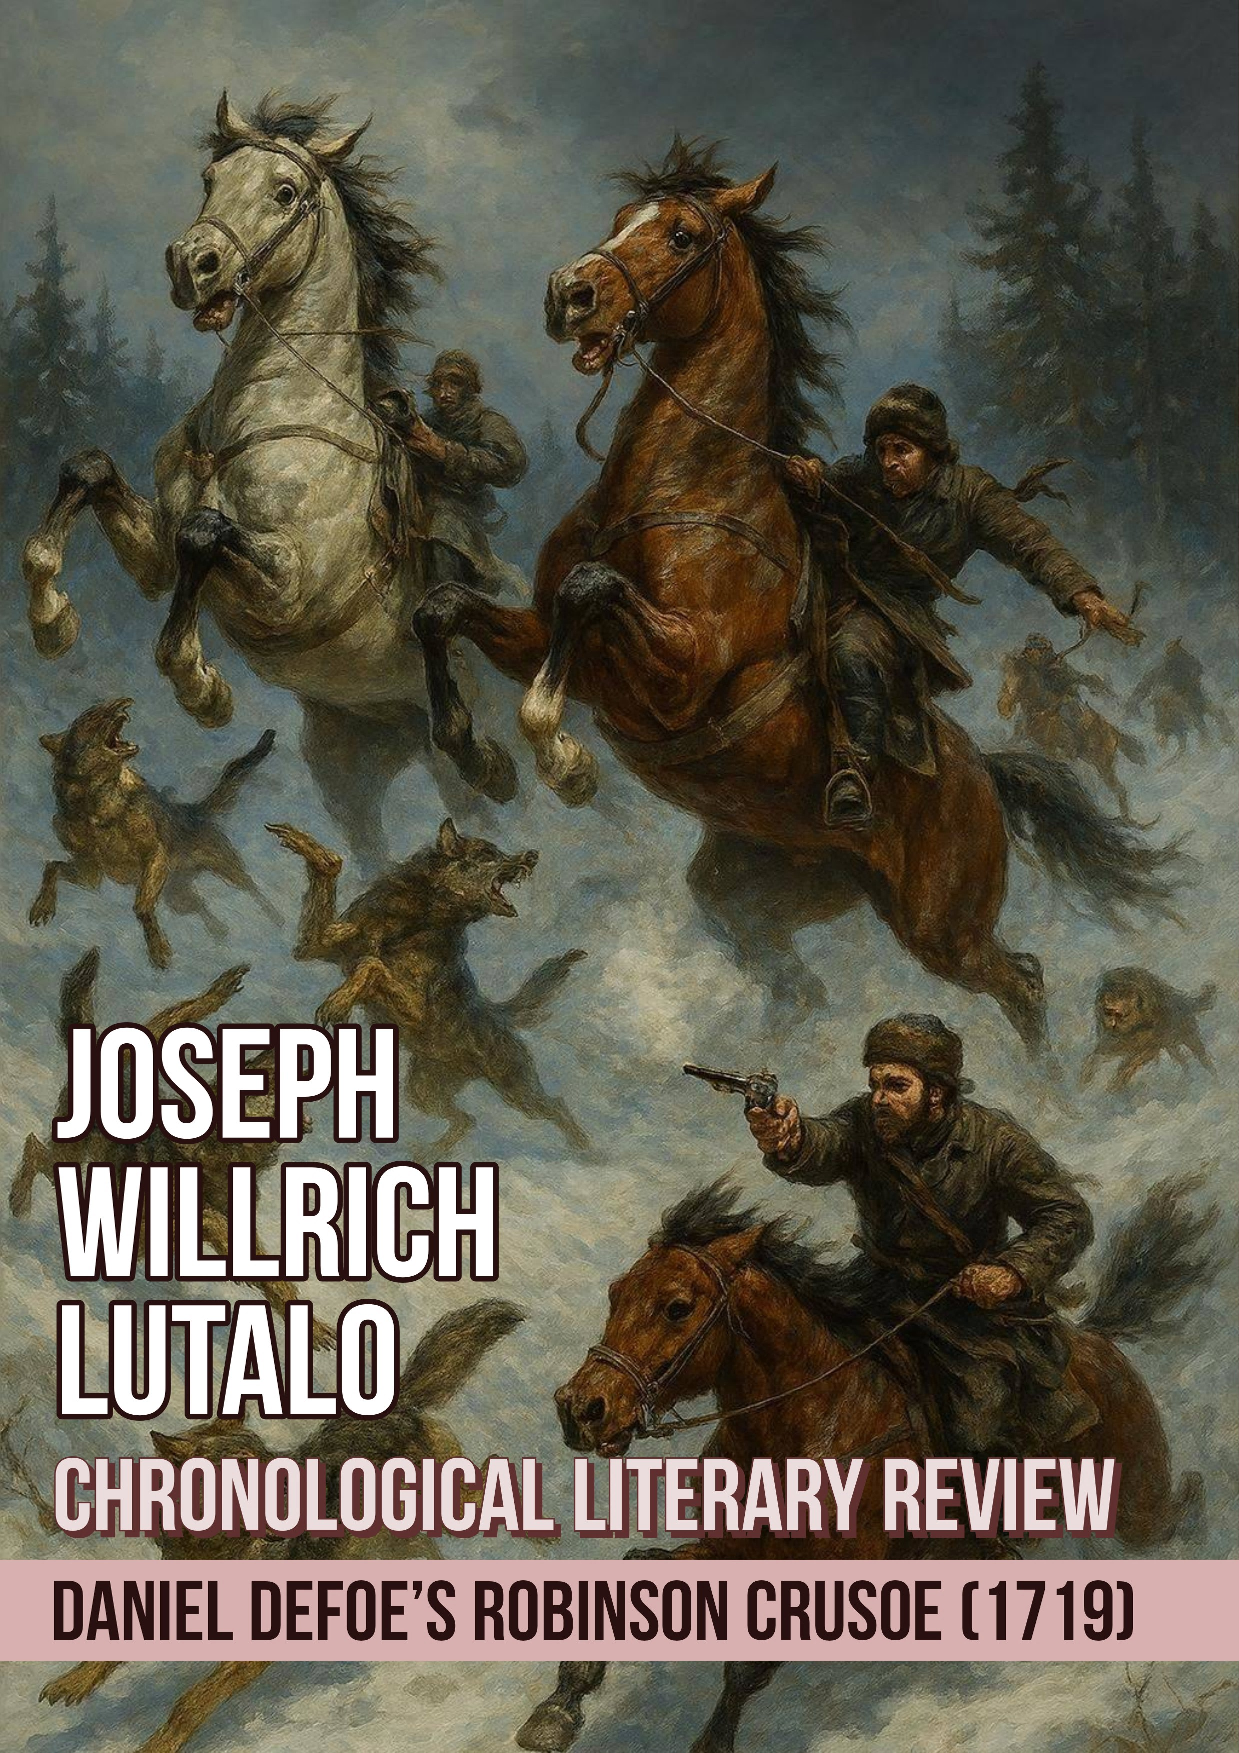
\includepdf[pages=1,
  width=\paperwidth,
  height=\paperheight,
  pagecommand={}]{resources/pdfs/frontcover.pdf}



\maketitle
\begin{abstract}
This paper presents a chronological literary review of Daniel Defoe's 1719 classic novel \textit{Robinson Crusoe} by his student and modern novelist, J. Willrich Lutalo, author of 2025 literary fiction novel, \textit{Rock `N' Draw}. It is compiled over an extended period of reflective reading spanning longer than a year; between February 2025 and May 2026. The review is structured as a series of dated notes, each capturing the precise moment of engagement with the text, accompanied by excerpts from the novel and personal commentary. This method allows for a layered exploration of the novel's themes, narrative techniques, and cultural resonances, while also documenting the evolving perceptions of the reader across more than a year of study.  

By situating the review within a temporal framework, the work highlights how sustained, reflective reading can deepen understanding of canonical literature. The inclusion of excerpts alongside commentary provides a dialogic interplay between Defoe's text and contemporary reflection, offering insights into the enduring relevance of \textit{Robinson Crusoe}. Ultimately, this review demonstrates the value of chronological annotation as both a scholarly and creative practice, producing a record that is at once analytical, personal, and historically conscious.  
 \newline\newline
     \textbf{Keywords}: Daniel Defoe, Robinson Crusoe, Reflective Reading, Canonical Literature, Chronological Literary Review
\end{abstract}


\section{Preamble}


As a writer, still furthering my craft but also as one that has without doubt read and encountered several other writers much greater than myself – both ancients and contemporaries, I have come to appreciate that it surely is true that without learning from others, there is little worthwhile contributions in literature that one would make. While writing a review of his work shall come another day, I have recently picked up a wonderful non-fiction work by the novelist (and fiction writer) I dearly admire; Stephen King. In his \textit{On Writing} \cite{King2000}, King puts it better than I would, when he says:



\noindent
\begin{minipage}{1\textwidth}
\vspace{1em}
\begin{quotation}
{\ttfamily

If you want to be a writer, you must do two things above all others: read a lot and write a lot. There's no way around these two things that I'm aware of, no shortcut.

\vspace{1em}

If you don't have time to read, you don't have the time (or the tools) to write. Simple as that.

}
\hspace*{\fill} ---\textbf{Stephen King}, \textit{On Writing}, 2000\cite{King2000}
\end{quotation}
\vspace{1em}
\end{minipage}


The writing of this current review happens to have started more than a year ago; on February 6th, 2025, at around the time I was winding up writing my second full-length novel, \textit{Rock `N' Draw} \cite{lutalo2025rock}. It was during the writing of that work, a wartime literary fiction novel situated in the Uganda of 2036 --- essentially, in the future, when I decided to revisit an `ancient' classic I'd already encountered many years before as a teenager. 

The original edition of \textbf{Daniel Defoe}'s adventure story came to me while I was in my late teens --- most likely around nineteen or so. However, despite having been into reading classics for a while, it somewhat did not resonate well with me, and so I quickly dumped it for more modern, `pulp fiction' works (the \textbf{Dan Brown}s, \textbf{David Icke}s, etc.) Moreover, before encountering Defoe for the first time, I'd already devoured some thick classics without illustrations in them such as \textbf{Homer}'s \textit{Odyssey} ($\sim$700 BC); a book I picked from a private collection at home --- mum loved reading too. Further, and despite having abandoned the school subject ``Literature" in my junior high-school after quitting the traditional catholic school \texttt{St. Henry's College Kitovu}, I did have the chance to read \textbf{Charles Dicken}'s \textit{Great Expectations} (1860) as part of my essential class load during Senior Two.

It is against that background that I returned to Daniel Defoe. Early 2025 while scouting about for some extra reading material to inspire my on-going work, I did come across a special edition of his classic curated, expanded and annotated by a team at Oxford University Press; Thomas Keymer and James Kelly. A modern rendition \cite{Defoe2007} presented under the ``Oxford World's Classics" series, the electronic-book quickly caught my attention as being paramount for me to read, and thus my journey revisiting Robinson Crusoe's tale begun.

In the rest of this review then, we shall focus on the reading journey I sustained for a little more than a year between February 6th 2025 and May 23rd 2026. We shall have each review session sectioned under the corresponding date and time, perhaps [optionally] annotated by an illustrative subtitle or concept-keyword, and then shall have this followed by a verbatim excerpt from the book, my notes or reflections on the material as well as any other essential review material I see fit to include. This style of review should especially help those that have already encountered Defoe's story to readily follow along, in nearly the order the story unfolds in \cite{Defoe2007}. Moreover, since both the reading and review process spanned a long period, the chronological presentation should help highlight and stress the special impact the book had on me during the course of my reading it, as well as how my appreciation of Defoe's masterpiece changed or morphed over time. Without doubt, newcomers to both Daniel Defoe, but also to literary reviews should likewise find much to takeaway from this ambitious\footnote{``Ambitious" because, despite being a lifelong lover of literature and especially fiction works, and also having penned several of my own --- short-stories, poetry, free-verse, essays, novellas, novels as well as music lyrics --- I can't pretend to be an authority on the matter just yet. I have no degree in literature, have not spent much time around PhDs nor professors of either English or Literature, and so, I strongly advise any reviewers or critics of my review to take my work with a grain of salt. Please, note that I surely welcome all kinds of criticism from readers of this work.} undertaking. 

%draw horizontal line
\noindent\rule{\textwidth}{0.4pt}

\section*{ABOUT REVIEWER}
\label{SECAGOUT}

% --- Lead with author image wrapped on the left, text flows to the right ---
\begin{wrapfigure}{L}{0.42\textwidth}
  \vspace{-6pt}
  \centering
  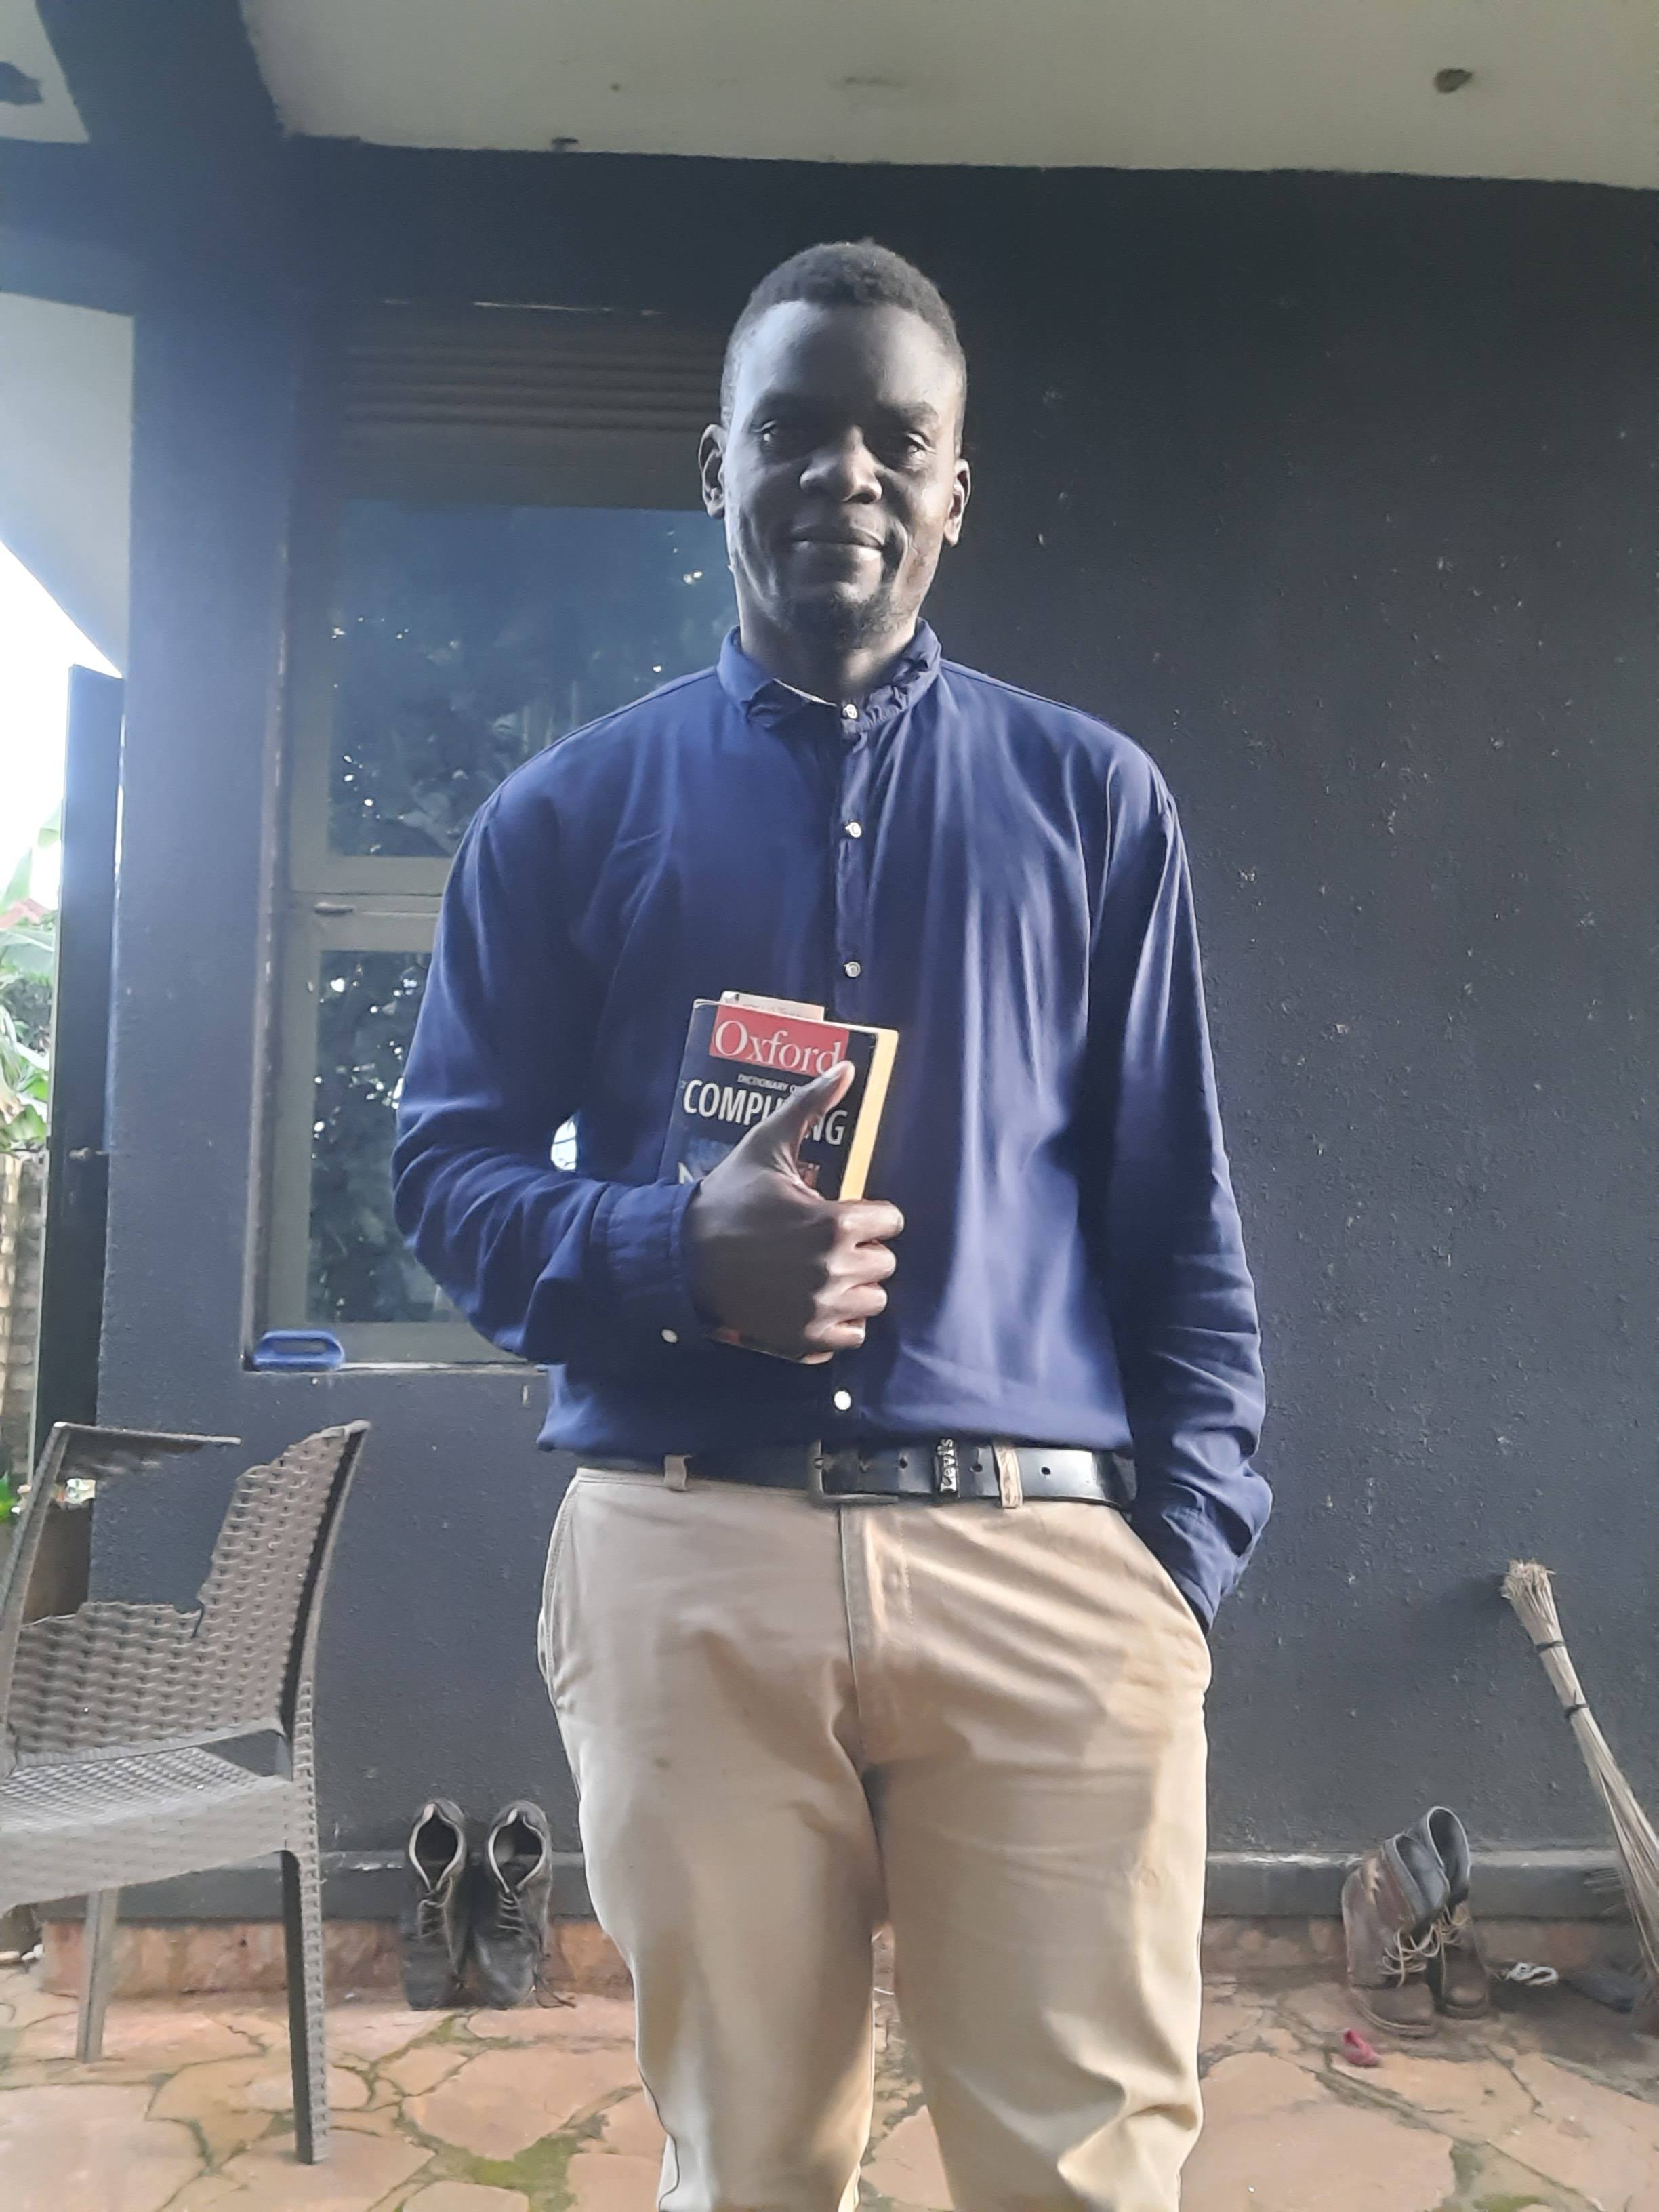
\includegraphics[width=0.40\textwidth]{resources/images/author.jpg} % replace with your filename
  \caption*{\small \textbf{Fut. Prof. Joseph W. Lutalo} at Nuchwezi Research}
  \vspace{-6pt}
\end{wrapfigure}

\texttt{[Future Professor]} \textbf{Joseph Willrich Lutalo} is an independent empirical researcher but also a seasoned theorist in software language engineering, esoteric science and mathematics. He's an avid writer on all things relating to modern scientific illuminism such as practical chaos magick, technomancing, occult art and crafts.  As of this moment, he is based at his private, personal laboratory known as ``Nuchwezi Research” in Garuga, UGANDA --- also home to the (mostly online) school: Nuchwezi Esoteric School (NES; \url{https://iona.nuchwezi.com}). He is the founder of an underground esoteric community of researchers and practitioners known as IoNA (Illuminates of Nuchwezi Angellic).  Otherwise, he was recently (2025) a finalist graduate researcher at Makerere University’s College of Computing and Information Sciences (CoCIS), from where he completed his MSc. Software Engineering and Data Communications. His Master’s thesis, ``VOSA: A Reusable and Reconfigurable Voice Operated Support Assistant Chatbot Platform" was successfully presented at SE2024 in Copenhagen, Denmark, and it introduced a hands-free human support tool driven by user-configurable knowledge models based on QAKBs.  

Since founding \textbf{Nuchwezi} ( \url{https://nuchwezi.com} ), a research-oriented technology service provider based in UGANDA, circa 2014, he has made extensive contributions in the form of mobile and web applications, software libraries, a new general-purpose programming language (TEA – \url{https://tea.nuchwezi.com} ) and several other contributions in both the arts and sciences. He has a total of 60+ academic works (ORCID), 20+ scholarly articles (Google Scholar) and has contributed a total of 150+ mini-lectures on several topics in computer science, maths and software engineering as well as two special lists focused on Occult Science (54 videos) and Chaos Magick (145 videos) (YouTube). Joseph has written 2 full-length novels as of this moment, and 3 novellas. Apart from being the brains and hands behind several unconventional musical acts based in Uganda and especially over ICs (\texttt{Internet Communities}) such as pioneer melodic metal-on-keys band MAZERA, underground Hip Hop acts Nemesis Fixx, Arch L, Mensa ICE, BATEMBUZYI and more, he also is the founder and Editor-in-Chief of \textbf{I*POW}, the Telegram-based \textit{International Internet Portfolio of Writers}. Fut. Prof. JWL continues to push the edge for what's possible in both fiction and non-fiction, written, spoken and performed modern [world] literature as and when the need arises. At 40 years of age as of May 2026, Joseph is likewise exploring the prospect of obtaining their PhD from potentially the University of Oxford.
\\\\
For Details on New and Old Scholarly Works Refer to ACADEMIA:\\ \url{https://mak.academia.edu/JosephWillrichLutalo}
\\\\
For Details on New and Old Creative Works Refer to YOUTUBE:\\ \url{https://YouTube.com/@1JWL}


%draw horizontal line
\noindent\rule{\textwidth}{0.4pt}

%\printbibliography

\bibliographystyle{unsrt}
\bibliography{References}

% inner cover
% or explicitly stretch to page size
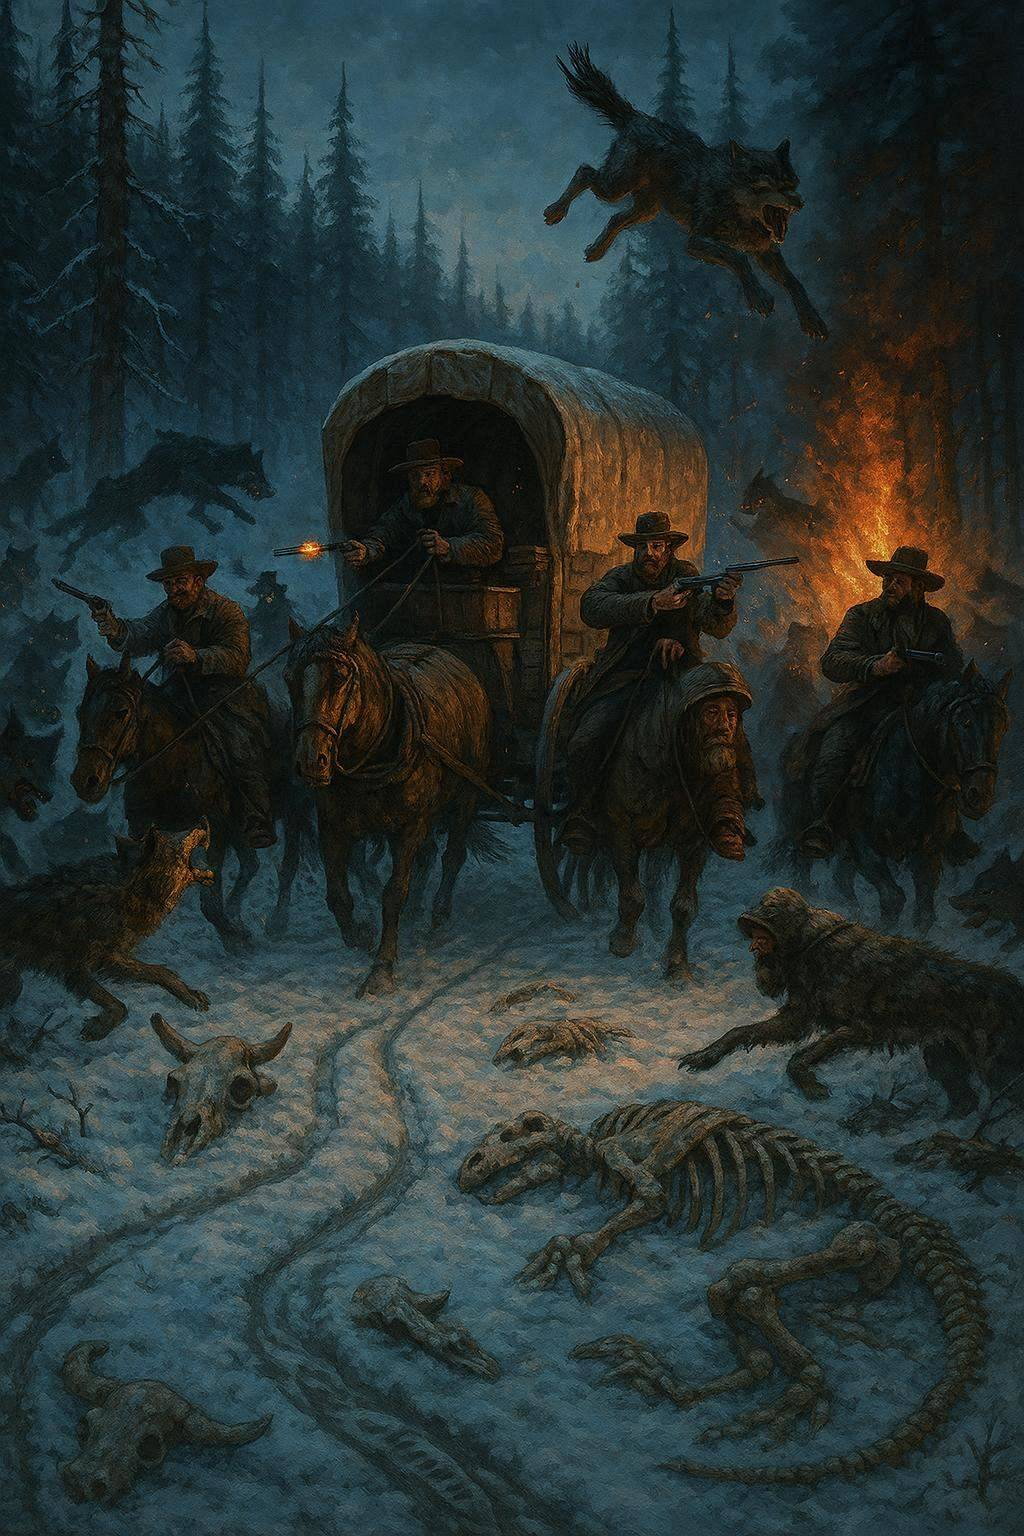
\includepdf[pages=1,
  width=\paperwidth,
  height=\paperheight,
  pagecommand={}]{resources/images/innercover_a.jpeg}


% inner cover
% or explicitly stretch to page size
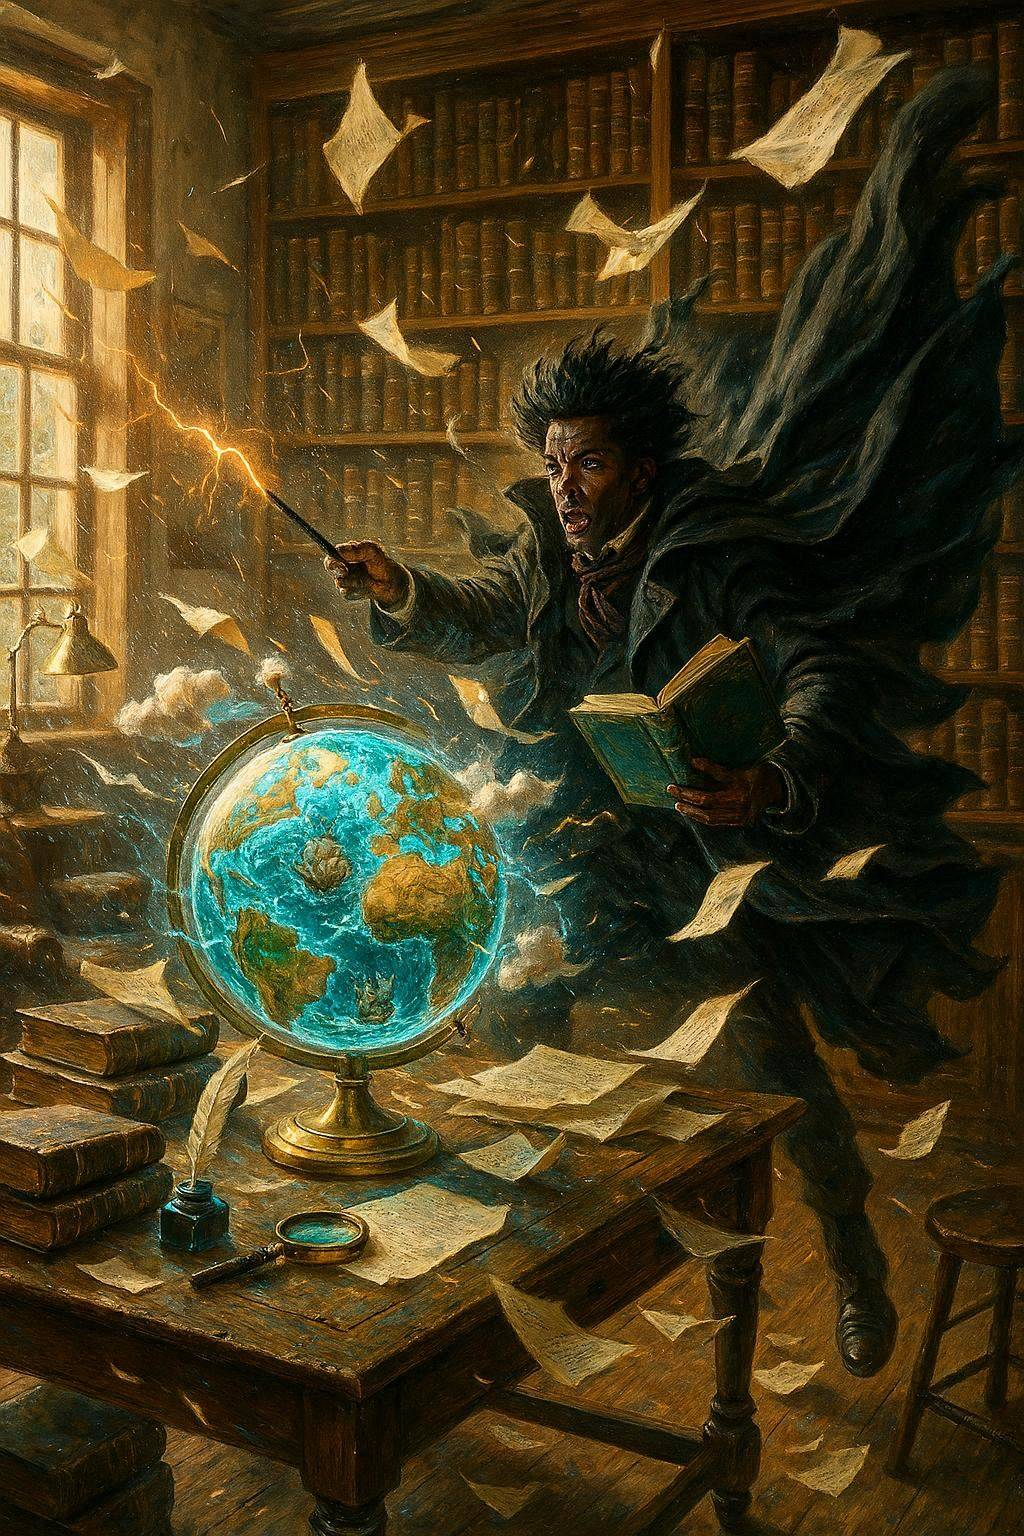
\includepdf[pages=1,
  width=\paperwidth,
  height=\paperheight,
  pagecommand={}]{resources/images/innercover_b.jpeg}


% insert [back] cover --- could just be a PNG or PDF
%
\includepdf[pages=1]{resources/pdf/backcover.pdf}

% or explicitly stretch to page size
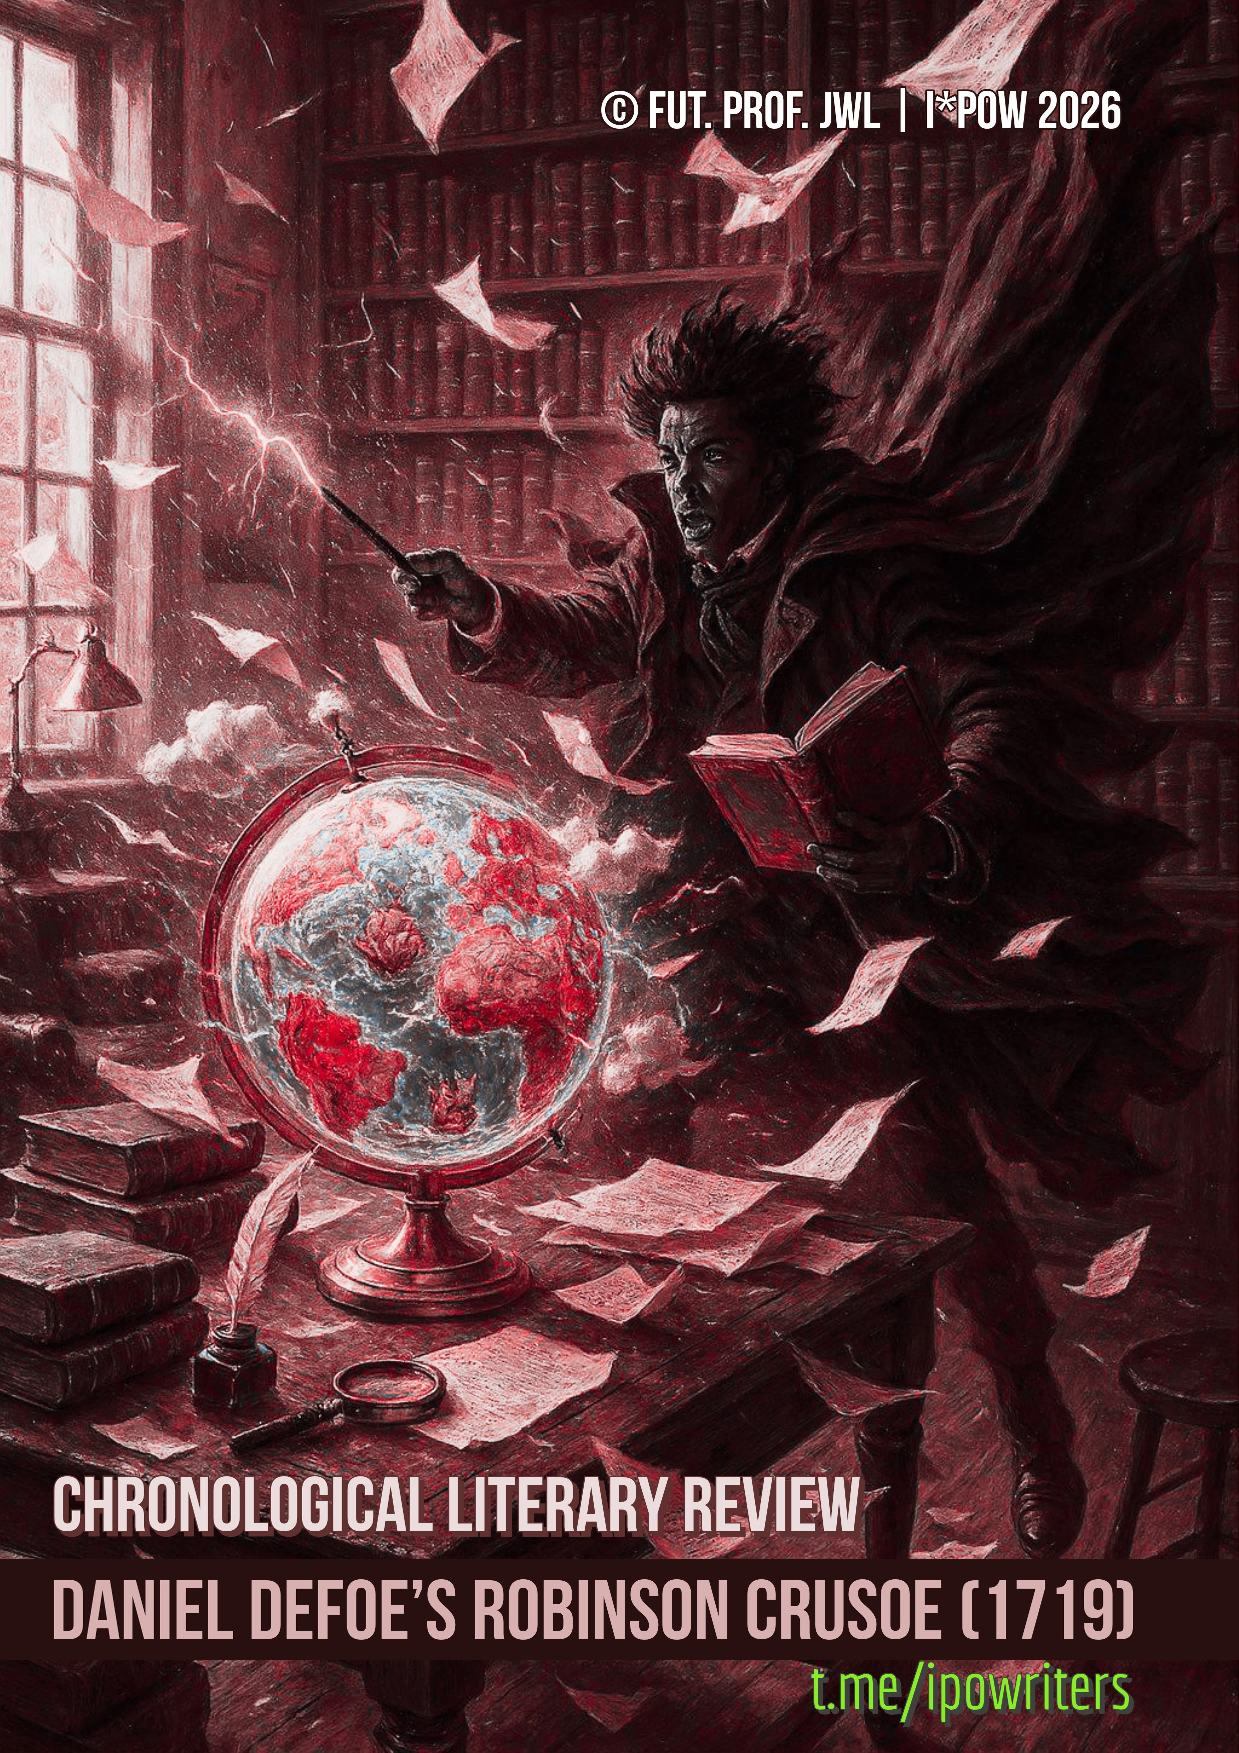
\includepdf[pages=1,
  width=\paperwidth,
  height=\paperheight,
  pagecommand={}]{resources/pdfs/backcover.pdf}

\end{document}